\documentclass{beamer}
\usetheme{Rochester}
\usecolortheme{orchid}
\useinnertheme{rounded}
\usepackage[T1]{fontenc}
\usepackage{lmodern}
\usepackage{amsmath}
\usepackage{tikz}
\setbeamertemplate{navigation symbols}{}
\setbeamertemplate{footline}[frame number]

% Change the course name, lecture number and topic.
\title{Lecture 5: Probability Basics}
\subtitle{STAT 101, Introduction to Statistics}
\author{Dr. Priya Natarajan}
\date{Week 3, Autumn Term}

\begin{document}

\begin{frame}
  \titlepage
\end{frame}

\begin{frame}{Today you will learn to}
  \begin{enumerate}
    \item Describe a sample space and events.
    \item Compute probabilities of simple events.
    \item Use the addition rule.
  \end{enumerate}
  \vspace{1em}
  \begin{block}{Before class}
    Read Chapter 4, sections 4.1 and 4.2.
  \end{block}
\end{frame}

\begin{frame}{Key definitions}
  \begin{definition}[Sample space]
    The set $S$ of all possible outcomes of an experiment.
  \end{definition}
  \begin{definition}[Event]
    Any subset $A \subseteq S$.
  \end{definition}
  \begin{block}{Equally likely outcomes}
    \[ P(A) = \frac{\text{number of outcomes in } A}{\text{number of outcomes in } S} \]
  \end{block}
\end{frame}

\begin{frame}{Worked example}
  \begin{exampleblock}{Rolling one die}
    What is the probability of rolling an even number?
  \end{exampleblock}
  % Each \pause reveals the next step when presenting.
  \pause
  \begin{itemize}
    \item $S = \{1,2,3,4,5,6\}$, so $|S| = 6$.
    \pause
    \item $A = \{2,4,6\}$, so $|A| = 3$.
    \pause
    \item $P(A) = 3/6 = 1/2$.
  \end{itemize}
\end{frame}

\begin{frame}{The addition rule}
  \begin{theorem}
    For any events $A$ and $B$:
    \[ P(A \cup B) = P(A) + P(B) - P(A \cap B) \]
  \end{theorem}
  \begin{columns}[c]
    \begin{column}{0.45\textwidth}
      \centering
      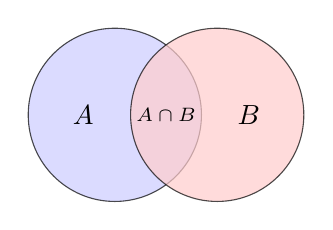
\begin{tikzpicture}
        \draw[fill=blue!20, opacity=0.7] (0,0) circle (1.1);
        \draw[fill=red!20, opacity=0.7] (1.3,0) circle (1.1);
        \node at (-0.4,0) {$A$};
        \node at (1.7,0) {$B$};
        \node[font=\scriptsize] at (0.65,0) {$A\cap B$};
      \end{tikzpicture}
    \end{column}
    \begin{column}{0.5\textwidth}
      \begin{alertblock}{Common mistake}
        Forgetting to subtract the overlap counts it twice.
      \end{alertblock}
    \end{column}
  \end{columns}
\end{frame}

\begin{frame}{Quick quiz}
  A card is drawn from a standard deck. What is $P(\text{heart or king})$?
  \vspace{1em}
  % Edit the answer options. The correct one turns green on the second click.
  \begin{enumerate}[A.]
    \item $17/52$
    \item<1-|alert@2> $16/52$
    \item $13/52$
    \item $4/52$
  \end{enumerate}
  \vspace{1em}
  \uncover<2>{
    \begin{exampleblock}{Answer: B}
      $13/52 + 4/52 - 1/52 = 16/52$, since the king of hearts is counted twice.
    \end{exampleblock}
  }
\end{frame}

\begin{frame}{Summary and homework}
  \begin{columns}[T]
    \begin{column}{0.48\textwidth}
      \begin{block}{Remember}
        \begin{itemize}
          \item $0 \le P(A) \le 1$
          \item $P(S) = 1$
          \item Subtract overlaps
        \end{itemize}
      \end{block}
    \end{column}
    \begin{column}{0.48\textwidth}
      \begin{block}{Homework}
        Problems 4.3, 4.7 and 4.12.\\
        Due next Tuesday.
      \end{block}
    \end{column}
  \end{columns}
\end{frame}

\end{document}
